\providecommand{\additionalOptionsForClass}{}
\documentclass[
  accentcolor=tud1c,	% Color theme for TUD corporate design
  colorbacktitle,		% Titlepage has colored background for title area
  inverttitle,			% Font color of title on titlepage is inverted
  \additionalOptionsForClass
  %german%,
  %twoside
]{tudexercise}

\parindent1em
%\parskip2ex

\usepackage[ngerman]{babel}
\usepackage[utf8]{inputenc}
\usepackage{listings}
\usepackage{booktabs}
\usepackage{amsmath}
\usepackage{algorithm2e}
\usepackage{hyperref}
\usepackage{xspace}
\usepackage{tabularx}
\usepackage{tikz}
\usepackage{cleveref}
\usepackage{numprint}
\usepackage{paralist}
\usepackage{verbatim}
\usepackage{tocloft} % for manipulating the table of contents

\usetikzlibrary{shapes}
\usetikzlibrary{calc}
\usetikzlibrary{arrows}
\usetikzlibrary{decorations}

\usepackage{pifont}
\newcommand{\cmark}{\ding{51}\xspace}%
\newcommand{\xmark}{\ding{55}\xspace}%

\usepackage{todonotes}
%\usepackage[disable]{todonotes} % Use this line to hide all todos

\definecolor{commentgreen}{RGB}{50,127,50}
\lstloadlanguages{C++,[gnu]make}
\lstset{language=C++}
\lstset{captionpos=b}
\lstset{tabsize=3}
\lstset{breaklines=true}
\lstset{basicstyle=\ttfamily}
\lstset{columns=flexible}
\lstset{keywordstyle=\color{purple}}
\lstset{stringstyle=\color{blue}}
\lstset{commentstyle=\color{commentgreen}}
\lstset{otherkeywords=\#include}
\lstset{showstringspaces=false}
\lstset{keepspaces=true}
\lstset{xleftmargin=1cm}
\lstset{literate=%
	{Ö}{{\"O}}1
	{Ä}{{\"A}}1
	{Ü}{{\"U}}1
	{ß}{{\ss}}2
	{ü}{{\"u}}1
	{ä}{{\"a}}1
	{ö}{{\"o}}1
	{'}{{\textquotesingle}}1
}

\lstnewenvironment{lstmake} %
{\lstset{language=[gnu]make}} %
{}


\newcommand{\superscript}[1]{\ensuremath{^{\textrm{#1}}}}
\newcommand{\subscript}[1]{\ensuremath{_{\textrm{#1}}}}

\newcommand{\setHeader}[1]{
\providecommand{\examheadertitle}{TODO: Titel einbinden}
\renewcommand{\examheadertitle}{#1}
\begin{examheader}
    \examheadertitle
\end{examheader}
}

\newcommand{\hints}[1]{
\paragraph*{Hinweise}
	\begin{itemize}
		\setlength{\itemsep}{0pt}
		#1
	\end{itemize}
}

\newcommand{\optional}{\xspace(optional)}
\newcommand{\experimental}{\xspace(experimentell)}

\usepackage{fancybox}
\newcommand{\optionaltextbox}{
	\bigskip
	\begin{center}
		\ovalbox{\parbox{0.98\textwidth}{Die Klausur kann ohne diese Aufgabe bestanden werden. Wir empfehlen aber sie trotzdem zu bearbeiten.}}
	\end{center}
}
\newcommand{\experimentaltextbox}{
	\bigskip
	\begin{center}
		\ovalbox{\parbox{0.98\textwidth}{Diese Aufgabe wurde neu erstellt und kann noch Fehler und Inkonsistenzen enthalten. Falls euch etwas derartiges auffällt sprecht uns bitte darauf an oder stellt es auf GitHub in den Issuetracker unter \url{https://github.com/Echtzeitsysteme/tud-cpp-exercises/issues}}}
	\end{center}
}

\newcommand{\enquote}[1]{\glqq#1\grqq\xspace}
\newcommand{\filename}[1]{\texttt{#1}}

\newcommand{\RK}[1]{\todo[]{\textbf{RK:} #1}}
\newcommand{\RKi}[1]{\todo[inline]{\textbf{RK:} #1}}

\newcommand{\ExercisePrefix}[1]{$[$#1$]$ \xspace}
\newcommand{\ExercisePrefixBasics}{\ExercisePrefix{G}}
\newcommand{\ExercisePrefixMemory}{\ExercisePrefix{S}}
\newcommand{\ExercisePrefixObjectOrientation}{\ExercisePrefix{O}}
\newcommand{\ExercisePrefixAdvanced}{\ExercisePrefix{F}}
\newcommand{\ExercisePrefixEmbeddedC}{\ExercisePrefix{C}}
\newcommand{\ExercisePrefixElevator}{\ExercisePrefix{A}}
\newcommand{\ExercisePrefixAdditionalInformation}{\ExercisePrefix{Z}}


\newcommand{\exday}{3}

\cppSetTitle

\begin{document}

\cppSetHeaderAndMakeTitle

\section{Vererbung und Polymorphie}
\subsection{Klasse \texttt{Person}}
Implementiere eine Klasse \texttt{Person}, die eine Person mit einem Namen darstellt.
Füge allen Konstruktoren und Destrukoren eine Ausgabe auf die Konsole hinzu, um später den Lebenszyklus der Objekte besser nachvollziehen zu können.

\begin{lstlisting}
class Person {
public:
	Person(const std::string& name);		// initialize the name of the person
	~Person();									// destructor
	std::string getInfo() const;			// get the name of the person
protected:
	std::string name;							// the name of the person
};
\end{lstlisting}

\hints{
	\item Verwende \texttt{\#include <string>} um \texttt{std::string} zu verwenden.
	\item Um ein String-Literal an eine \texttt{std::string} Variable anzuhängen, musst du aus dem String-Literal zuerst ein \texttt{std::string}-Objekt machen: \texttt{std::string text = std::string("Name: " ) + name;}.
}

\subsection{Klasse \texttt{Student}}
Implementiere eine Klasse \texttt{Student}, die von \texttt{Person} erbt (\texttt{public}) und einen Studenten mit einer Matrikelnummer (ebenfalls \texttt{std::string}) modelliert.
Rufe in der Initialisierungsliste den entsprechenden Konstruktor der Elternklasse \texttt{Person} mittels \texttt{Person(name)} auf.
Füge allen Konstruktoren und Destrukoren eine Ausgabe auf die Konsole hinzu, um später den Lebenszyklus der Objekte besser nachvollziehen zu können.

\begin{lstlisting}
class Student: public Person {	// public inheritance
public:
	Student(const std::string& name, const std::string& studentID); // init name and ID
	~Student();							// destructor
	std::string getInfo() const;	// override Person::getInfo() - get name and studentID
private:
	std::string studentID;			// the student ID of the student
};
\end{lstlisting}

\hints{
	\item Erst ab C++11 gibt es die Möglichkeit mit dem Schlüsselwort \texttt{override} zu deklarieren, dass eine Funktion eine andere (virtuelle) überschreibt (vergleichbar mit der Annotation \texttt{@Override} in Java). Trotzdem zeigt dir Eclipse mit einem kleinen aufwärts zeigenden Dreieck links neben den Zeilennummern an, ob du eine Methode überschreibst oder nicht.
	\item Du kannst bei Bedarf die \texttt{getInfo()}-Implementation der Elternklasse \texttt{Person} von \texttt{Student} aus mittels \texttt{Person::getInfo()} aufrufen.
}

\subsection{Test}
Erstelle nun in \texttt{main()} je eine Person und einen Studenten und gib deren Daten auf der Konsole aus.
Vergewissere dich, dass bei \texttt{Student} auch die Matrikelnummer ausgegeben wird.
Schau dir auch die Ausgaben der Konstruktoren und Destruktoren an, und versuche, diese nachzuvollziehen.

Implementiere dann folgende Funktion und teste deine Implementation erneut, indem du \texttt{printPersonInfo()} mit beiden Personentypen aufrufst.

\begin{lstlisting}
void printPersonInfo(const Person *person);		// print person information on console
\end{lstlisting}

\hints{
	\item Dadurch dass \texttt{Person} als \texttt{const} Zeiger übergeben wird, können auch Unterklassen von \texttt{Person}, wie z.B. \texttt{Student}, übergeben werden. 
}


\subsection{Dynamic Dispatch bei \texttt{printPersonInfo}}
Du merkst, dass \texttt{printPersonInfo()} unabhängig von übergebenem Personentyp immer nur den Namen der Person ausgibt, aber nicht die Matrikelnummer.
Der Grund dafür ist, dass \texttt{getInfo()} nicht als \texttt{virtual} deklariert wurde und deshalb auch kein dynamischer Dispatch der Methode stattfindet.
Deklariere daher \texttt{getInfo()} in beiden Klassen als \texttt{virtual}.

Teste deine Implementation erneut und vergewissere dich, dass nun immer die richtige Methode aufgerufen wird.

\hints{
	\item Möchte man Methoden einer Basisklasse überschreiben, \textbf{muss} \texttt{virtual} in der Basisklasse gesetzt werden. In den abgeleiteten Klassen kann \texttt{virtual} weggelassen werden, es wird dann vom Compiler ergänzt.
}

\subsection{Virtueller Destruktor}
Lege einen Studenten mit \texttt{new} dynamisch auf dem Heap an und speichere die Adresse in einem Zeiger auf eine \texttt{Person}.
Lösche die Person anschließend mit \texttt{delete}.

\begin{lstlisting}
	Person *pTim = new Student("Tim", "321654");
	delete pTim;
\end{lstlisting}

Analysiere die Konsolenausgabe.
Es wird nur der Destruktor von \texttt{Person} aufgerufen, obwohl es sich um ein Objekt vom Typ \texttt{Student} handelt.
Auch hier liegt es daran, dass kein dynamischer Dispatch bei der Zerstörung erfolgt.
Deklariere deshalb in beiden Klassen den Destruktor als \textbf{virtual} und teste die Korrektheit der Destruktoraufrufe.

\hints{
	\item Faustregel: Besitzt eine Klasse mindestens eine virtuelle Funktion, so sollte auch der Destruktor virtuell sein.
}



\newpage

\section{Pure Virtual}
In dieser Aufgabe wollen wir Vererbung und Polymorphie dazu nutzen, um mathematische Ausdrücke als Bäume von Primitivoperationen zu modellieren.
Dazu werden wir eine abstrakte Oberklasse \texttt{Expression} mit der abstrakten Methode \texttt{compute()} erstellen.
Einzelne Knotentypen wie Addition und Subtraktion werden von \texttt{Expression} abgeleitet und implementieren \texttt{compute()}, um die jeweilige Operation zu realisieren.
\begin{figure}[h]
\begin{center}
	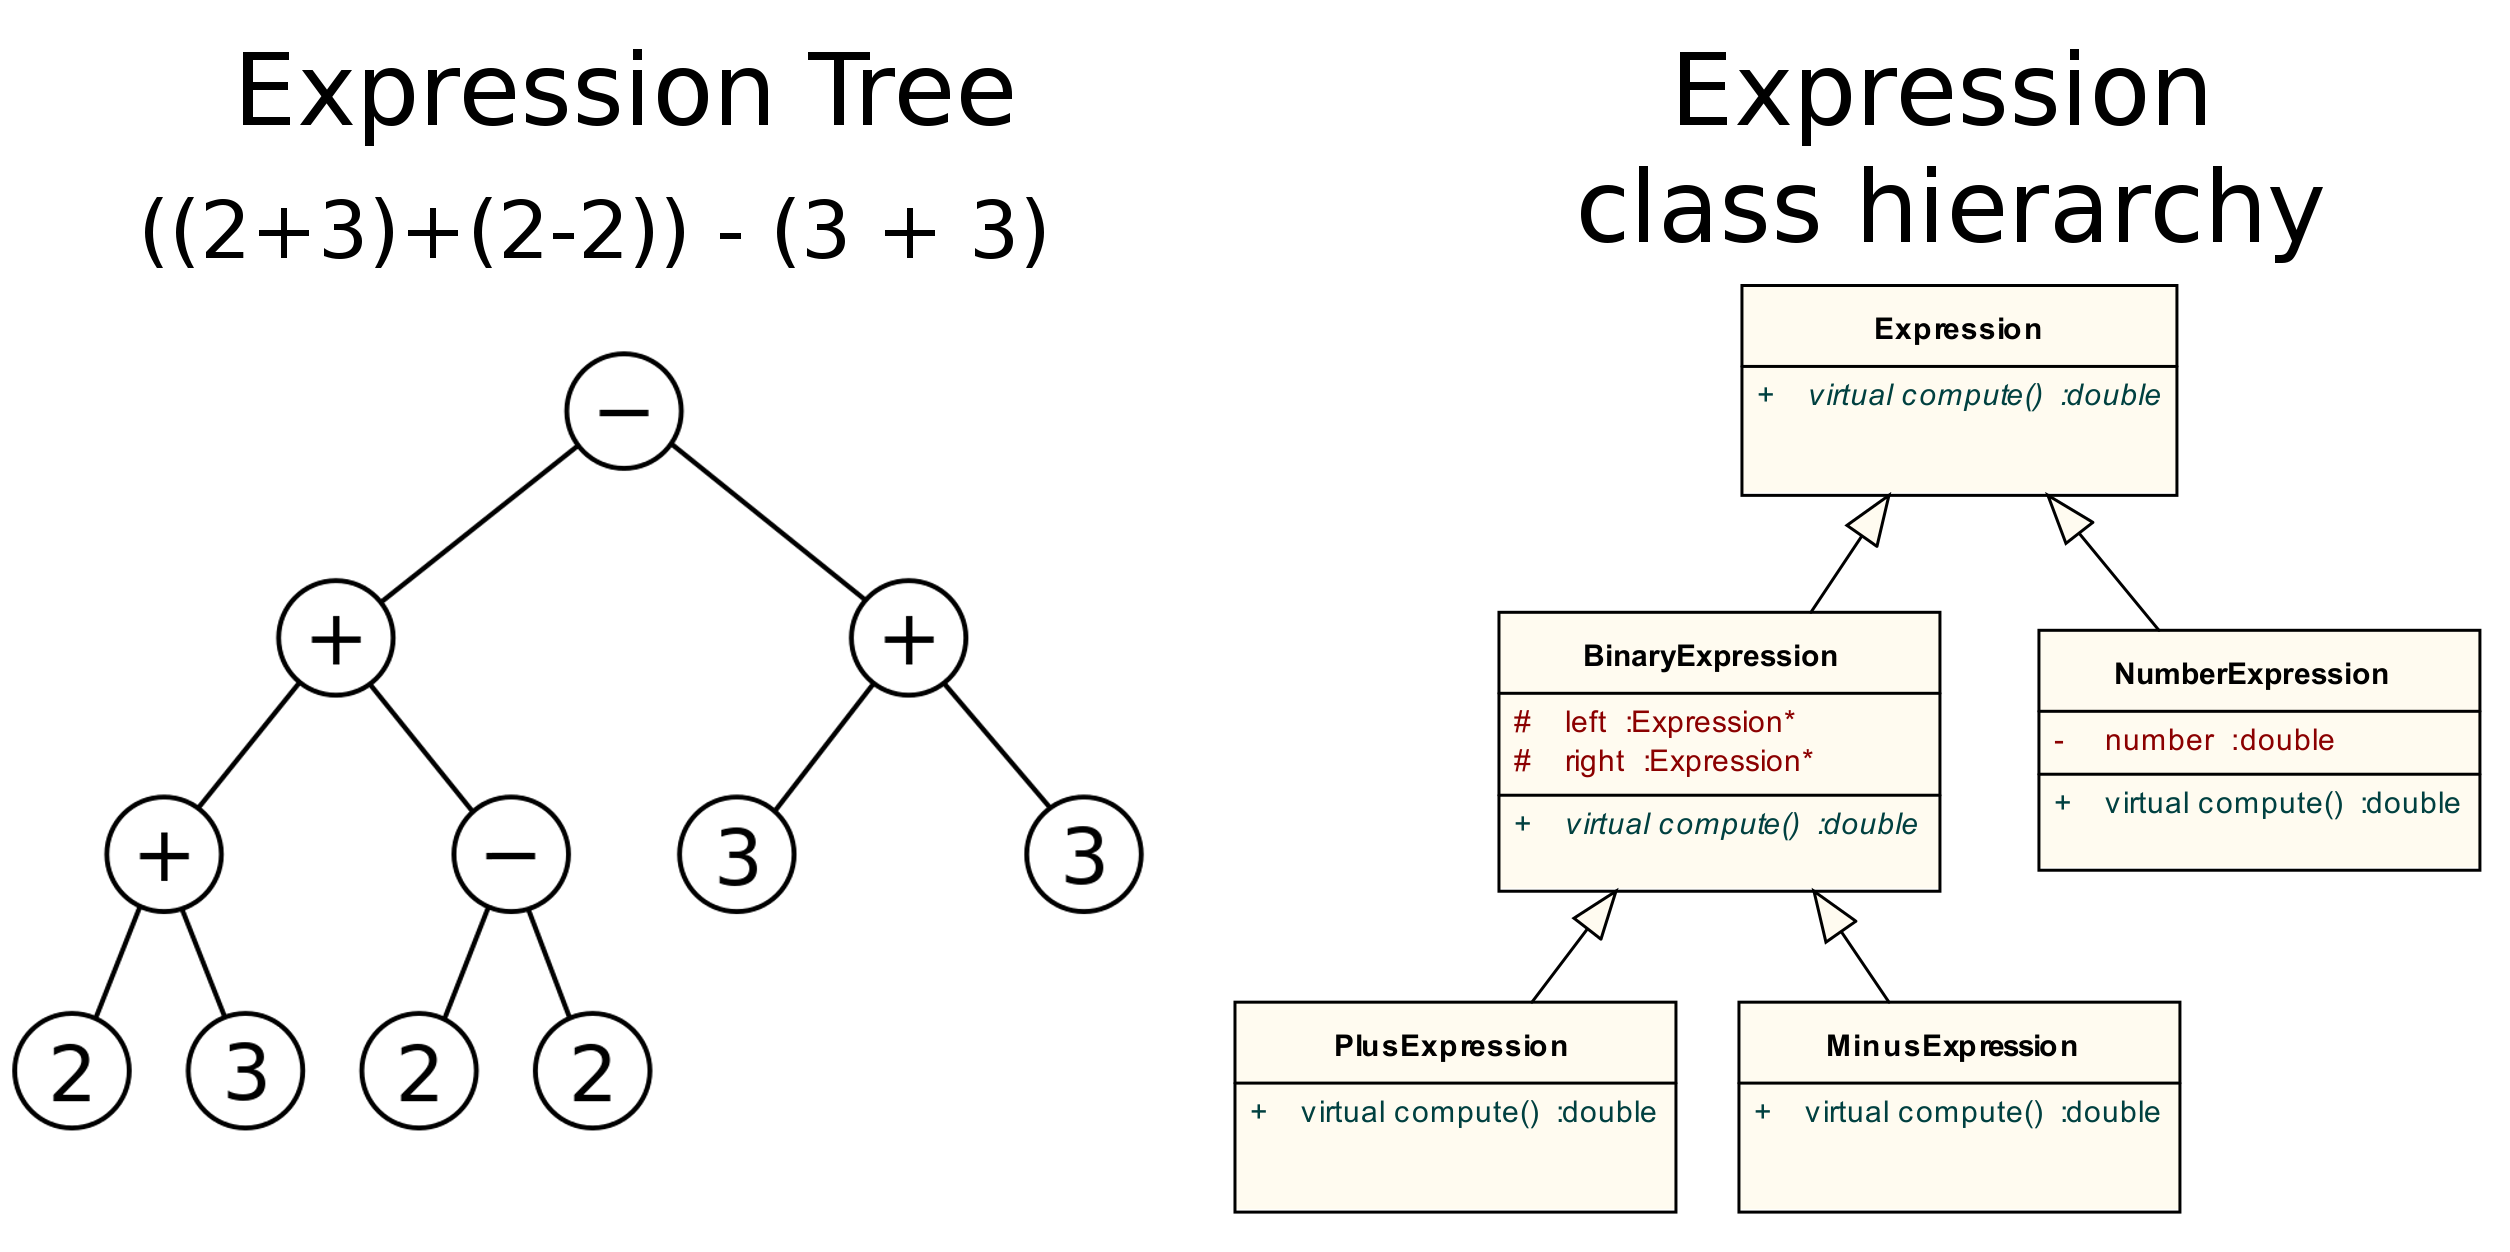
\includegraphics[width=.75\textwidth]{figures/ExpressionTree.png}\\
	\caption{Abbildung: Beispielausdruck mit Ausdrucksbaum und Klassenhierarchie}
\end{center}
\end{figure}


\begin{enumerate}

\item \textbf{Klasse \texttt{Expression}}
Schreibe die abstrakte Klasse \texttt{Expression}.
Diese soll als Basisklasse für alle Ausdrücke dienen.
Implementiere einen parameterlosen Konstruktor und einen virtuellen Destruktor, die je eine Meldung auf der Konsole ausgeben, sodass es bei der Ausführung ersichtlich wird, wann eine \texttt{Expression} erzeugt und wann zerstört wird.
Deklariere außerdem eine abstrakte (pure \texttt{virtual}) Methode \texttt{virtual double compute() = 0;}, die das Ergebnis des Ausdrucks berechnen und zurückgeben soll. 

\item \textbf{Klasse \texttt{NumberExpression}}
Schreibe die Klasse \texttt{NumberExpression}, die ein (Baum-)Blatt mit einer Zahl darstellt.
Dementsprechend soll \texttt{NumberExpression} von \texttt{Expression} erben und ein Attribut zum Speichern einer Zahl besitzen, das im Konstruktor initialisiert wird.
Implementiere den Konstruktor und virtuellen Destruktor und versehe auch diese mit einer Konsolenausgabe.
Die Methode \texttt{compute()} gibt die gespeicherte Zahl zurück.

\item \textbf{Klasse \texttt{BinaryExpression}}
Schreibe die abstrakte Klasse \texttt{BinaryExpression} mit den \texttt{protected} Attributen \texttt{Expression *left, *right}.
Implementiere den Konstruktor und virtuellen Destruktor mit entsprechender Ausgabe.
Vergiss nicht, im Destruktor die beiden Zweige zu löschen. 

\item \textbf{Klassen \texttt{Plus-} und \texttt{Minusexpression}}
Schreibe die Klassen \texttt{PlusExpression} und \texttt{MinusExpression}, die von \texttt{BinaryExpression} erben und eine Addition bzw. Subtraktion realisieren. 
Implementiere die Kon- und Destruktoren sowie die \texttt{compute()} Methode.

\item \textbf{Test}
Teste deine Implementation.
Ein gutes Beispiel findest du in Abbildung weiter oben.
Schaue dir die Ausgabe genau an und versuche anhand der gegebenen Klassenhierarchie die Reihenfolge der Erzeugung und Zerstörung von Objekten  nachzuvollziehen.

\end{enumerate}



\newpage

\section{Fortsetzung Aufzugsimulator}
Unser bisheriger Aufzugsimulator hat eine feste Strategie, nach der die einzelnen Stockwerke abgefahren werden. Mithilfe von Polymorphie können wir den Simulator so erweitern, dass die Strategie austauschbar wird.  

\subsection{Vorbereitung}
Lagere die bereits existierende Simulation des Aufzugs aus der \texttt{main}-Funktion in eine eigene Funktion \texttt{runSimulation()} aus. Die Funktion sollte das volle Gebäude als Parameter entgegennehmen und eine Liste (\texttt{std::list<int>}) der angefahrenen Stockwerke zurückgeben. Überlege dir, auf welche Art das Gebäude idealerweise übergeben werden sollte.
Teste deine Implementation.

\subsection{Klasse \texttt{ElevatorStrategy}}
Implementiere die Klasse \texttt{ElevatorStrategy}.
Diese soll die Basisklasse für verschiedene Aufzugstrategien sein.
Damit die Strategie das Gebäude nicht selbst modifizieren kann, wird \texttt{Building} per \texttt{const} Pointer übergeben.

\begin{lstlisting}
// Elevator strategy class: Determines to which floor the elevator should move next.
class ElevatorStrategy {
public:
	virtual ~ElevatorStrategy();
	virtual void createPlan(const Building*);		// create a plan for the simulation - the default implementation does nothing but saving the building pointer
	virtual int nextFloor() = 0;	// get the next floor to visit
protected:
	const Building *building;		// pointer to current building, set by createPlan()
};
\end{lstlisting}



\subsection{Eine einfache Aufzusstrategie}
Implementiere eine einfache Aufzugstrategie, indem du eine neue Klasse erzeugst die von \texttt{ElevatorStrategy} erbt.
Diese soll folgendermaßen vorgehen: 
Falls der Aufzug momentan leer ist, soll zum tiefsten Stockwerk gefahren werden, wo sich noch Personen befinden.
Falls der Aufzug nicht leer ist, wird das Zielstockwerk einer der Personen im Aufzug ausgewählt.

\subsection{Implementation von \texttt{runSimulation}}
Ändere nun \texttt{runSimulation()} entsprechend um, sodass die Simulation anhand der gegebenen Strategie durchgeführt wird.
Folgender Pseudocode kann dir als Denkhilfe dienen:

\begin{algorithm}[H]
 \SetAlgoLined
 \While{People in Building or Elevator}{
   Calculate next floor;\\
   
   Move Elevator to next floor; \\
   Let all arrived people off; \\
   Let all people on floor into Elevator;\\
 }
\end{algorithm}

Teste die einfache Aufzugstrategie

\subsection{Neue Aufzugstrategien (optional)}
Entwickle eine eigene Aufzugstrategien, indem du erneut eine neue Klasse erzeugst die von \texttt{ElevatorStrategy} erbt.
Versuche, verschiedene Größen zu optimieren, wie z.B. die Anzahl der Stopps oder die verbrauchte Energie.
Hierfür könnte Backtracking verwenden\footnote{Siehe \url{http://de.wikipedia.org/wiki/Backtracking}}, eine einfache Methode, um eine optimale Lösungen durch Ausprobieren zu finden. Beachte, dass der Aufzug auch kopiert werden kann, um verschiedene Strategien zu testen.


\end{document}
